% Электронный учебник будет представлять собой один файл в формате pdf.
% Для того, чтобы создать этот
% файл, нужно поработать с настоящим документом, который в дальнейшем будем называть
% <<рабочий файл>>. Прежде, чем приступать к работе, прочтите внимательно первые две части
% <<Руководства пользователю>>. По большому счету электронное издание <<Руководство
% пользователю>> показывает стиль и
% структуру создаваемого электронного учебника (стиль и структуру, конечно же, можно будет
% поменять по Вашему усмотрению). Основную часть экрана занимает так называемая рабочая
% область -- здесь будет представлена информация учебника, предназначенная для изучения
% студентами. Правая часть -- интерактивная панель, предназначенная для удобной навигации
% по документу.

% Теперь можно приступать к работе. Внимательно читайте все комментарии (они начинаются после
% символа %).
% Если Вы что-нибудь поменяли, то для того, чтобы увидеть результат,
% нужно скомпилировать рабочий файл в pdf-документ (см. <<Руководство пользователю>>).

%---------------------------------------------------------------------------------------------------------------

\documentclass[12pt, a4paper]{book}% Эту команду не стоит менять
\usepackage{xspace,colortbl}% Эту команду не стоит менять
\usepackage[utf8]{inputenc}% Эту команду не стоит менять
\usepackage[english,russian]{babel}% Эту команду не стоит менять
\usepackage{euscript,latexsym,amsfonts,amsthm,amsmath,amssymb}% Эту команду не стоит менять
\usepackage[pdftex,hypertex]{hyperref}% Эту команду не стоит менять
\usepackage{color}% Эту команду не стоит менять
\usepackage[screen,panelright,sectionbreak]{pdfscreen}% Эту команду не стоит менять
\graphicspath{{images/}{images/amblems/}{images/fon/}{images/panel/}{images/pic/}}% Эту
% команду не стоит менять. Она указывает путь к папкам, в которых хранятся графические файлы
 \margins{.25in}{.25in}{.25in}{.30in}% Эту команду не стоит менять
 \screensize{6.25in}{8in}% Эту команду не стоит менять
  \changeoverlay% Эту команду не стоит менять
\usepackage{longtable}% Эту команду не стоит менять

\usepackage{regexpatch}
\usepackage{listings}
\definecolor{keyword}{RGB}{0,0,150}
\definecolor{identifier}{RGB}{0,0,0}
\definecolor{comment}{RGB}{128,128,128}
\definecolor{string}{RGB}{0,128,0}
\definecolor{numbers}{RGB}{128,128,128}

\lstdefinestyle{customc}{
  belowcaptionskip=1\baselineskip,
  breaklines=true,
  frame=L,
  xleftmargin=\parindent,
  language=C++,
  showstringspaces=false,
  basicstyle=\small\ttfamily,
  numberstyle=\color{numbers},
  keywordstyle=\bfseries\color{keyword},
  commentstyle=\itshape\color{comment},
  identifierstyle=\color{identifier},
  stringstyle=\color{string},
}
\lstset{escapechar=@,style=customс}

\makeatletter
\xpatchcmd*\@Overlay@Hook{\put(\strip@pt\@tempdima,\strip@pt\@tempdima)}
{\put(\strip@pt\@tempdima,\strip@pt\dimexpr.5\paperheight)}{}{}
\makeatother

%--------------------------------------------------------------------------------------------

 \paneloverlay{but3.png}% Аргумент этой команды, записанный в фигурных скобках, можно
% изменить. <<{but3.png}>> -- это имя графического файла, который используется в качестве
% фона интерактивной панели. Здесь можно прописать имя любого рисунка в формате png или pdf,
% который Вы хотите использовать в качестве фона для интерактивной панели. Файл
% этого рисунка должен находиться в папке Images/Panel.

%---------------------------------------------------------------------------------------------------

\overlay{m1.png} % Аргумент этой команды, записанный в фигурных скобках, можно
% изменить. <<{m8.png}>> -- это имя графического файла, который используется в качестве
% фона основой рабочей области. Здесь можно прописать имя любого рисунка в формате
% png или pdf, который Вы хотите использовать в качестве фона для основной рабочей области.
% Файл этого рисунка должен находиться в папке Images/fon.

%---------------------------------------------------------------------------------------------

\def\panel{\begin{minipage}[t][\paperheight][t]{\panelwidth}% Эту команду не стоит менять
\centering\null\vspace*{12pt}% Эту команду не стоит менять
 \par\vspace{0.3cm}% Эту команду не стоит менять

%---------------------------------------------------------------------------------------------

\includegraphics[width=2.54cm]{favicon_ru_RU.png}\par\vspace{0.6cm}% Эта команда позволяет вставить
% любую картинку в качестве эмблемы в верхней части интерактивной панели. Аргумент команды
% в квадратных скобках <<[width=2.54cm]>> задает ширину эмблемы (в сантиметрах),
% а аргумент команды в фигурных скобках <<{univ.png}>> -- это имя графического файла,
% содержащего саму эмблему. Здесь можно прописать имя любого рисунка в формате
% png или pdf, который Вы хотите использовать в качестве эмблемы.
% Файл этого рисунка должен находиться в папке Images/amblems
\vspace{0mm}% Эта команда задает расстояние (в миллиметрах) до следующей после эмблемы строки
{\LARGE\itshape Кафедра}% Эту команду лучше не менять

{\large\itshape АСОИ}% Впишите сюда название Вашей кафедры

\vspace{5mm}% Эта команда задает расстояние (в миллиметрах) до первой кнопки
% интерактивной панели
%---------------------------------------------------------------------------------------------------

 \Acrobatmenu{FirstPage}{\addButton{1.05in}{\FBlack\@Начало}}\par\vspace{3mm} % Эта команда создает
% кнопку <<Начало>> на интерактивной панели. Нажатие этой кнопки возвращает пользователя
% на первую (титульную) страницу электронного учебника. Аргумент команды <<{\FBlack\@Начало}>>
% можно поменять (например, написать вместо <<Начало>> <<Пачатак>> или <<Титульная страница>>).

%------------------------------------------------------------------------------------------------

\hyperref[oglo]{{\addButton{1.05in}{\@Содержание}}}\par\vspace{3mm} %Эта команда создает
% кнопку <<Содержание>> на интерактивной панели. Нажатие этой кнопки возвращает пользователя
% на первую страницу раздела <<Содержание>> электронного учебника.
% Аргумент команды <<{\@Содержание}>> можно поменять (например, написать
% вместо <<Содержание>> <<Змест>> или <<Оглавление>>).

%---------------------------------------------------------------------------------------------

\hyperref[mybutton]{\addButton{1.05in}{\@Ваша кнопка}}\par\vspace{3mm}%Эта команда создает
% кнопку <<Ваша кнопка>> на интерактивной панели. Нажатие этой кнопки вернет пользователя
% на ту страницу электронного учебника, на которую Вы захотите. Для этого нужно в определенное
% Вами место любого раздела электронного учебника поставить метку \label{mybutton} (подробнее
% о метках можно прочитать в <<Руководстве пользователю>>). Обратите внимание, что имя этой
% метки должно совпасть с аргументом команды, записанном
% в квадратных скобках (\hyperref[mybutton]).
% Аргумент команды <<{\@Ваша кнопка}>> нужно поменять (написать
% вместо <<Ваша кнопка>> любой текст, указывающий пользователю, какую информацию он
% получит, нажав на эту кнопку). Такого типа кнопки удобно создавать для быстрого
% доступа пользователя к некоторой информации электронного учебника (например, справочной
% информации, перечню формул, и т.д.). При желании таких кнопок можно создать несколько
% (сколько позволит высота Интерактивной панели). Для этого нужно соответствующее
% число раз скопировать и вставить сразу после этого комментария
% команду \hyperref[imyametki]{\addButton{1.05in}{\@Ваша кнопка}}\par\vfill
% Если же Вы не хотите создавать ни одной своей кнопки, удалите всю строку, содержащую
% описываемую здесь команду и весь текст данного комментария.

%--------------------------------------------------------------------------------------------

\Acrobatmenu{PrevPage}{\addButton{.51in}% Не меняйте эту команду. Она создает кнопку перехода
{\FBlack\scalebox{.8}[1.4]{\btl}}}\hspace{1pt}% на одну страницу назад
\Acrobatmenu{NextPage}{\addButton{.51in}% Не меняйте эту команду. Она создает кнопку перехода
{\LBlack\scalebox{.8}[1.4]{\rtl}}}\par\vspace{3mm}% на одну страницу вперед

%---------------------------------------------------------------------------------------------

\Acrobatmenu{FirstPage}{\addButton{.51in}% Не меняйте эту команду. Она создает кнопку быстрого
{\FBlack\scalebox{.8}[1.4]{\btl\btl}}}\hspace{1pt}% перехода на первую страницу
\Acrobatmenu{LastPage}{\addButton{.51in}% Не меняйте эту команду. Она создает кнопку быстрого
{\LBlack\scalebox{.8}[1.4]{\rtl\rtl}}}\par\vspace{3mm}% перехода на последнюю страницу

%---------------------------------------------------------------------------------------------

\Acrobatmenu{GoToPage}{\addButton{1.05in}% Не меняйте эту команду. Она создает кнопку,
{\@Страница~\thepage~\@из~\pageref*{pages_total}}}\par\vspace{3mm}% позволяющую совершать
% переход на любую страницу электронного учебника

%---------------------------------------------------------------------------------------------

\Acrobatmenu{GoBack}{\addButton{1.05in} {\@Назад}}\par\vspace{3mm}% Не меняйте эту команду. Она
% создает удобную кнопку возврата к той странице электронного учебника, с которой был совершен
% переход по любой гиперссылке текста учебника или по некоторой кнопке Интерактивной панели.
% Аргумент команды <<{\@Назад}>> можно поменять (например написать вместо <<Назад>>
% <<Обратно>> или <<Возврат>>).

%---------------------------------------------------------------------------------------------------

\Acrobatmenu{FullScreen}{\addButton{1.05in}{\@На весь экран}}\par\vspace{3mm}% Эту команду лучше
% не менять. Она создает кнопку, позволяющую <<развернуть>> электронный учебник на весь экран.
% Аргумент команды <<{\@На весь экран}>> можно поменять (например написать вместо
% <<На весь экран>> <<Развернуть>> или <<Увеличить>>)

%---------------------------------------------------------------------------------------------

\Acrobatmenu{Quit}{\addButton{1.05in}{\@Закрыть}}\par\vspace{3mm}% Эту команду лучше
% не менять. Она создает кнопку, нажатие которой закрывает электронный учебник. Аргумент
% команды <<{\@Закрыть}>> можно поменять (например написать вместо
% <<Закрыть>> <<Выход>> или <<Уйти>>)

%---------------------------------------------------------------------------------------------

\end{minipage}}% Эту команду не стоит менять

\definecolor{panelbackground}{gray}{.8}% Эту команду не стоит менять
  \definecolor{buttonbackground}{gray}{.9}% Эту команду не стоит менять
  \definecolor{buttonshadow}{gray}{.2}% Эту команду не стоит менять
  \definecolor{orange}{rgb}{1,.549,0}% Эту команду не стоит менять
  \definecolor{orange1}{rgb}{1,.5,0}% Эту команду не стоит менять
  \definecolor{section0}{rgb}{0,.5,.1}% Эту команду не стоит менять
  \definecolor{section1}{rgb}{0,.5,1}% Эту команду не стоит менять
  \definecolor{section2}{rgb}{0,.5,.5}% Эту команду не стоит менять
  \definecolor{section3}{rgb}{0,.5,.4}% Эту команду не стоит менять
  \definecolor{section4}{rgb}{.4,.5,.2}% Эту команду не стоит менять
  \definecolor{section5}{rgb}{.5,.5,.3}% Эту команду не стоит менять
\newcommand{\esup}{\mathop{\rm ess\:sup\;}_{t>0\;\,}}% Эту команду не стоит менять
\newcommand{\res}{\mathop{\rm res}}% Эту команду не стоит менять
\renewcommand{\Re}{{\rm Re}}% Эту команду не стоит менять
\renewcommand{\Im}{\operatorname{Im}}% Эту команду не стоит менять
\newcommand{\norm}[1]{\left\Vert#1\right\Vert}% Эту команду не стоит менять
\newcommand{\set}[1]{\left\{#1\right\}}% Эту команду не стоит менять
\newcommand{\h}{{\mathcal H}}% Эту команду не стоит менять
\newcommand{\nur}{\EuScript{L}_{\nu,r}}% Эту команду не стоит менять
\newcommand{\nutwo}{\EuScript{L}_{\nu,2}}% Эту команду не стоит менять
\newcommand{\eqdef}{\stackrel{\rm def}{=}}% Эту команду не стоит менять
\renewcommand{\thesection}{\arabic{chapter}.\arabic{section}\hspace{-4mm}}% Эти команды не стоит менять
\renewcommand{\thesubsection}{\arabic{chapter}.\arabic{section}.% Эту команду не стоит менять
\arabic{subsection}\hspace{-4mm}}% Эту команду не стоит менять
\renewcommand{\theequation}{\arabic{chapter}.\arabic{equation}}% Эту команду не стоит менять
\makeatletter% Эту команду не стоит менять
\newcommand*\l@struct{\@dottedtocline{1}{0em}{2.3em}}% Эту команду не стоит менять
\newcommand{\l@abcd}[2]{\rightskip=\@pnumwidth\leftskip=% Эту команду не стоит менять
\@tempdima\hspace{-2.7em}\noindent #1\hfill% Эту команду не стоит менять
\rlap{\makebox[\@pnumwidth][r]{\bf#2}}}% Эту команду не стоит менять
\renewcommand*\l@section{\@dottedtocline{1}{1.5em}{2.2em}}% Эту команду не стоит менять
\renewcommand*\l@subsection{\@dottedtocline{2}{3.8em}{3.0em}}% Эту команду не стоит менять
\renewcommand{\section}{\@startsection{section}{1}{1pt}% Эту команду не стоит менять
{4.0ex plus -0.2ex minus -0.2ex}{2.0ex plus 0.2ex}{\centering\bf}}% Эту команду не стоит менять
\renewcommand{\subsection}{\@startsection{subsection}{2}% Эту команду не стоит менять
{23pt}{3.5ex plus -0.2ex minus -0.2ex}{1ex plus 0.2ex}{\bf}}% Эту команду не стоит менять
\renewcommand{\chapter}{\vspace{8mm}\global\@topnum=0% Эту команду не стоит менять
\@afterindenttrue\secdef\@chapter\@schapter}% Эту команду не стоит менять
\renewcommand{\@makechapterhead}[1]{{\parindent=0pt\raggedright% Эту команду не стоит менять
\bf ЛЕКЦИЯ { }\centering\Large\thechapter\vspace{0.1mm}~\centering% здесь можно заменить
% слово <<ЛЕКЦИЯ>> на любое другое

\large\bf #1\par\nopagebreak\vspace{4mm}}}% Эту команду не стоит менять

\renewcommand{\tableofcontents}{\section*{\contentsname}\@starttoc{toc}}% Эту команду не
% стоит менять

%--------------------------------------------------------------------------------------------

% Следующие команды задают вид и структуру раздела <<Содержание>> (этот раздел
% генерируется автоматически).
\def\@chapter[#1]#2{\ifnum \c@secnumdepth >\m@ne% Эту команду не стоит менять
\if@mainmatter% Эту команду не стоит менять
\refstepcounter{chapter}% Эту команду не стоит менять
\typeout{\@chapapp\space\thechapter.}% Эту команду не стоит менять
\addcontentsline{toc}{chapter}% Эту команду не стоит менять
{{\rm Лекция \,\thechapter}\ \ #1}% Здесь можно заменить слово <<Лекция>> на любое другое
\else% Эту команду не стоит менять
\addcontentsline{toc}{chapter}{#1}% Эту команду не стоит менять
\fi% Эту команду не стоит менять
\else% Эту команду не стоит менять
\addcontentsline{toc}{chapter}{#1}% Эту команду не стоит менять
\fi% Эту команду не стоит менять
\chaptermark{#1}% Эту команду не стоит менять
\addtocontents{lof}{\protect\addvspace{10\p@}}% Эту команду не стоит менять
\addtocontents{lot}{\protect\addvspace{10\p@}}% Эту команду не стоит менять
\if@twocolumn% Эту команду не стоит менять
\@topnewpage[\@makechapterhead{#2}]% Эту команду не стоит менять
\else% Эту команду не стоит менять
\@makechapterhead{#2}% Эту команду не стоит менять
\@afterheading% Эту команду не стоит менять
\fi}% Эту команду не стоит менять

\makeatother% Эту команду не стоит менять

%--------------------------------------------------------------------------------------------

% Следующие команды определяют имена окружений типа <<Теорема>> (см. <<Руководство
% пользователю>>).
% Аргумент команды \newtheorem, записанный в фигурных скобках -- это имя окружения,
% которое будет использоваться при записи команды, создающей соответствующее окружение
% в тексте электронного учебника, а поэтому оно должно состоять из латинских символов;
% команда \color{red} задает цвет надписи имени окружения на русском языке
% (доступные цвета: red (красный), gray (серый), orange (оранжевый), blue (голубой),
% green (зеленый) и т.д).
% Можно создавать свои собственные окружения такого типа. Например, команда
% \newtheorem{mymicl}{\indent \color{red}Моя мысль}[chapter] создаст окружение
% типа <<Теорема>> с именем <<Моя мысль>>.
\newtheorem{theorem}{\indent \color{red}Теорема}[chapter]
\newtheorem{lemma}{\indent \color{red}Лемма}[chapter]
\newtheorem{corollary}{\indent \color{red}Следствие}[chapter]
\newtheorem{note}{\indent \color{red}Замечание}[chapter]
\newtheorem{opr}{\indent \color{red}Определение}[chapter]
\newtheorem{example}{\indent \color{red}Пример}[chapter]
\newtheorem{utv}{\indent \color{red}Утверждение}[chapter]
\newtheorem{gip}{\indent \color{red}Гипотеза}[chapter]
\newtheorem{way}{\indent \color{red}Способ}[chapter]

%--------------------------------------------------------------------------------------------

\pagestyle{empty}% Эту команду не стоит менять



% Теперь вся подготовительная работа проведена, стиль и структура электронного
% учебника заданы. Дальше можно начинать наполнение электронного учебника.

% -----------------------------------------------------------------------------------------

\begin{document}\large% Эту команду не стоит менять
% Приступим к созданию титульной страницы. Далее можно менять все, что написано
% на русском языке. Но не забывайте читать комментарии.
\begin{center}% Эту команду не стоит менять. Она <<центрирует>> текст, заключенный между
% командами \begin{center} и \end{center}, по ширине экрана.
  УЧРЕЖДЕНИЕ ОБРАЗОВАНИЯ\\
  <<Брестский государственный технический университет>>
\end{center}% Эта команда завершает <<центрирование>> текста
\vspace{20mm}% Эта команда увеличивает расстояние между строками (расстояние указано
% в фигурных скобках в миллиметрах).
\begin{center}% Эту команду не стоит менять. Она <<центрирует>> текст, заключенный между
% командами \begin{center} и \end{center}, по ширине экрана.
\textbf{% Эта команда задает полужирный шрифт текста, являющегося аргументом
% команды (т.е. текста, заключенного в фигурные скобки)
     {\LARGE \color{red} СИСТЕМНОЕ ПРОГРАММНОЕ ОБЕСПЕЧЕНИЕ}\\[10mm]% Переход на следующую строку
% задан командой \\, а в квадратных скобках указано расстояние
% до следующей строки текста (в миллиметрах).
    \\[10mm]% Переход на следующую строку задан командой \\,
% а в квадратных скобках указано расстояние до следующей строки текста (в миллиметрах).
    {\it\Large Электронный учебно-методический комплекс }\\% Переход на следующую строку
% задан командой \\
    {\it\Large для студентов факультета электронно-информационных систем}% Любую из строк такого вида можно
% при желании удалить или добавить новую с произвольным текстом.
}
\end{center}% Эта команда завершает <<центрирование>> текста
\vspace{30mm}% Эта команда увеличивает расстояние между строками (расстояние указано
% в фигурных скобках в миллиметрах).
\begin{center}% Эту команду не стоит менять. Она центрирует текст, заключенный между
% командами \begin{center} и \end{center}, по ширине экрана.
Брест\\% Переход на следующую строку задан командой \\
БрГТУ\\% Переход на следующую строку задан командой \\
  2023% Здесь указывается год создания электронного учебника
\end{center}% Эта команда завершает <<центрирование>> текста

% --------------------------------------------------------------------------------------------

\newpage% Эта команда задает переход на новую страницу (разрыв страницы).

% На этой странице будет размещена информация об авторах, рецензентах, экспертах и т.д.
% Прежде, чем приступать к работе с этой страницей,
% прочитайте часть 3 <<Руководства пользователю>>.

 \overlay{m1.png}% Эта команда задает новый фон рабочей области. Аргумент этой команды,
% записанный в фигурных скобках, можно  изменить. <<{m1.png}>> -- это имя графического
% файла, который используется в качестве фона основой рабочей области. Здесь можно
% прописать имя любого рисунка в формате png или pdf, который Вы хотите использовать
% в качестве фона для основной рабочей области.
% Файл этого рисунка должен находиться в папке Images/fon.

{\large% Эта команда задает шрифт определенного размера (см. <<Руководство пользователю>>)
\begin{flushleft}% Эту команду не стоит менять. Она выравнивает по левому краю текст,
% заключенный между командами \begin{flushleft} и \end{flushleft}.
 {\bf\color{red} Авторы:}% Здесь можно прописать любой текст (например, заменить слово
% <<Авторы>> на <<Авторы-составители>>

% Ниже команды \bf задают полужирный шрифт текста в группе, заключенной в фигурные скобки

~~~~{\bf Алексей Кивака} 




\vspace{10mm}% Эта команда увеличивает расстояние между строками (расстояние указано
% в фигурных скобках в миллиметрах).

{\bf\color{red}Рецензенты:}%Здесь можно прописать любой текст (например, заменить слово
% <<Рецензенты>> на <<Эксперты>>

~~~~{\bf Фамилия Имя Отчество} -- должность

 ~~~~{\bf Фамилия Имя Отчество} -- должность
\end{flushleft}% Эта команда завершает выравнивание текста по левому краю.

\vspace{10mm}% Эта команда увеличивает расстояние между строками (расстояние указано
% в фигурных скобках в миллиметрах).


%-------------------------------------------------------------------------------------------------

\newpage% Эта команда задает переход на новую страницу (разрыв страницы).

% На этой странице мы зададим автоматическую генерацию раздела <<Содержание>> электронного
% учебника

\paneloverlay{but3.png}% Аргумент этой команды, записанный в фигурных скобках, можно
% изменить. <<{but3.png}>> -- это имя графического файла, который используется в качестве
% фона интерактивной панели. Здесь можно прописать имя любого рисунка в формате png или pdf,
% который Вы хотите использовать в качестве фона для интерактивной панели. Файл
% этого рисунка должен находиться в папке Images/Panel.

\overlay{overlay2.pdf}% Здесь мы снова меняем фон рабочей области.
% Аргумент этой команды, записанный в фигурных скобках, можно
% изменить. <<{overlay2.pdf}>> - это имя графического файла, который используется в качестве
% фона рабочей области. Здесь можно прописать имя любого рисунка в формате
% png или pdf, который Вы хотите использовать в качестве фона для основной Рабочей области.
% Файл этого рисунка должен находиться в папке Images/fon.

\renewcommand{\contentsname}{СОДЕРЖАНИЕ}% Здесь можно слово <<Содержание>> заменить на любое
% другое (например <<Оглавление>>)

\addtocontents{toc}% Эту команду не стоит менять.
\large\tableofcontents\large\label{oglo}% Эту команду не стоит менять.

\newpage% Эта команда задает переход на новую страницу (разрыв страницы).


%-----------------------------------------------------------------------------

\section*{Предисловие}% Эта команда начинает раздел <<Предисловие>>. Можно назвать этот раздел
% и по-другому.
\addcontentsline{toc}{struct}{Предисловие}% Эту команду не стоит менять. Она добавляет
% в раздел <<Содержание>> ссылку на раздел <<Предисловие>>.


%-------------------------------------------------------------------------------------------

\newpage % Эта команда начинает новую страницу

\section*{ПРИМЕРНЫЙ ТЕМАТИЧЕСКИЙ ПЛАН} % Эта команда начинает новый раздел. Его название (текст
% в фигурных скобках) можно поменять.
\addcontentsline{toc}{struct}{Примерный тематический план}% Эта команда добавляет название
% раздела в раздел <<Содержание>>. Если меняете название раздела в предыдущей команде,
% то точно также меняйте текст в фигурных скобках этой команды.
{\normalsize% Эта команда уменьшает шрифт текста на данной странице до стандартного.
\begin{center}% Эта команда центрирует текст, заключенный между \begin{center} и \end{center}
\begin{longtable}{|c|p{12cm}|c|c|}% Эта команда начинает многостраничную таблицу (см. часть 4
% <<Руководства пользователю>>). Если Вас устраивает структура предлагаемой таблицы, не
%меняйте эту команду
\hline% Эта команда рисует горизонтальную линейку.
~ & ~ & ~ & ~  \\% Здесь вставлена пустая строка.
№ & \multicolumn{1}{|c|}{\bf Название  темы, перечень } & ЛК & ПР  \\% Здесь можно менять
~ & \multicolumn{1}{|c|}{\bf изучаемых вопросов}  & ~  &  ~ \\% любой текст на русском языке.
% ЛК -- сокращение для <<Лекции>>, ПР -- сокращение для <<Практические занятия>>.
   ~ & ~ & ~ & ~  \\% Здесь вставлена пустая строка.
\hline% Эта команда рисует горизонтальную линейку.
% Дальше следует продолжение таблицы с содержанием примерного тематического плана.
% Ячейки таблицы отделяются друг от друга знаком &, строки таблицы отделяются друг от друга
% командой \\.
% Первый столбец -- порядковый номер. Второй столбец -- название темы и перечень
% изучаемых вопросов. Третий столбец -- количество часов лекций, отводимое на изучение темы.
% Четвертый столбец -- количество часов практических (лабораторных)  занятий.
1 & {\bf Название темы.} Перечень изучаемых вопросов & 2  & 2  \\
\hline % Эта команда рисует горизонтальную линейку.
2& {\bf Название темы.} Перечень изучаемых вопросов  & 2  & 4  \\
\hline % Эта команда рисует горизонтальную линейку.
3& {\bf Название темы.} Перечень изучаемых вопросов  & 2  & 2  \\
\hline % Эта команда рисует горизонтальную линейку.
4& {\bf Название темы.} Перечень изучаемых вопросов  & 2  & 2  \\
\hline % Эта команда рисует горизонтальную линейку.
5& {\bf Название темы.} Перечень изучаемых вопросов  & 2  & 2  \\
\hline % Эта команда рисует горизонтальную линейку.
6& {\bf Название темы.} Перечень изучаемых вопросов  & 2  & 2  \\
\hline % Эта команда рисует горизонтальную линейку.
7& {\bf Название темы.} Перечень изучаемых вопросов  & 2  & 2  \\
\hline % Эта команда рисует горизонтальную линейку.
8& {\bf Название темы.} Перечень изучаемых вопросов  & 2  & 2  \\
\hline % Эта команда рисует горизонтальную линейку.
% Можете добавлять или удалять любое количество строк.

\end{longtable}% Эта команда завершает таблицу
\end{center}}% Эта команда завершает центрирование текста

%---------------------------------------------------------------------------------------------

\newpage 
\chapter{Тема 21 Лексический, синтаксический, семантический анализ}

Компиляторы преобразуют операторы языка в машинные коды целиком для всей программы. В результате обработки исходного текста программы формируется объектный модуль, который затем может многократно выполняться после его загрузки в оперативную память.

Интерпретаторы осуществляют преобразование операторов в машинные коды во время выполнения программы. После запуска программы в оперативную память одновременно загружаются исходный текст программы, написанный на языке высокого уровня, и интерпретатор, который последовательно транслирует операторы программы и сразу же их выполняет.

В современных ЭВМ одни и те же языки программирования могут быть представлены как компилирующие или интерпретирующие системы программирования.

Интерпретирующие системы программирования эффективны на этапе разработки программ, так как минимизируют время на отладку. Применение режима интерпретации для многократного выполнения отлаженных программ нецелесообразно, так как интерпретатор занимает дополнительный объем оперативной памяти, а также из-за трансляции замедляется выполнение программы.

Компилирующие СП эффективны при регулярной эксплуатации программ, так как имеется уже готовый к выполнению объектный модуль, что экономит время, затрачиваемое на трансляцию, и место в оперативной памяти. Разработка и отладка программ с использованием компилятора связаны с дополнительными временными затратами на трансляцию всего текста при определении ошибки.

Компиляторы обычно несколько проще в реализации, чем интерпретаторы, кроме того, не каждый язык программирования допускает построение простого интерпретатора. Однако интерпретаторы имеют существенное преимущество перед компиляторами, которое долгое время не принималось во внимание: откомпилированный код всегда привязан к архитектуре вычислительной системы, на которую он ориентирован, в то время как исходный текст программы непосредственно связан только с семантикой языка программирования, которую проще стандартизировать.

В настоящее время с развитием глобальных вычислительных сетей и распространением всемирной сети Интернет вопрос о переносимости программ и их независимости от аппаратной платформы приобретает все большую актуальность. Поскольку в состав сети могут входить ЭВМ различной архитектуры, то требование единообразного выполнения текста исходной программы на каждой из этих ЭВМ становится определяющим. Язык описания гипертекста HTML (Hypertext Markup language), на основе которого функционирует сейчас практически вся структура сети Интернет, является интерпретируемым языком. Трансляторы языков Java и JavaScript сочетают в себе функции компиляции и интерпретации: текст исходной программы компилируется в некоторый промежуточный двоичный код, не зависящий от архитектуры вычислительной системы; этот код передается по сети и выполняется в режиме интерпретации на принимающей стороне.

\begin{figure}
\begin{center}
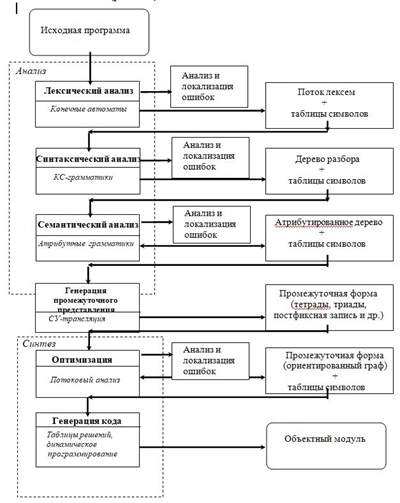
\includegraphics[width=250]{pic21-1}
\caption*{Обобщенная структура компилятора и основные фазы процесса компиляции}
\end{center}
\end{figure}

\begin{center}{\bfseries Лексический анализ}
\end{center}
  
\begin{opr}
  Лексический анализ (ЛА) - это первый этап процесса трансляции. Основная задача лексического анализа – разбить входной текст, состоящий из последовательности символов алфавита, на минимально значимые части языка, называемые лексемами. Лексемами естественных языков являются слова. В языках программирования встречаются лексемы различных типов, состав которых определяется синтаксисом конкретного языка программирования.
\end{opr}

Лексический анализ разбивает текст программы на указанные элементы. Особенность любой лексики — ее элементы представляют собой регулярные линейные последовательности символов. Например, идентификатор — это произвольная последовательность букв, цифр и символа «_», начинающаяся с буквы или «_». Лексика ЯП анализируется и интерпретируется на фазе лексического анализа при трансляции.

На фазе лексического анализа входная программа, представляющая собой поток литер, разбивается на лексемы – слова в соответствии с определениями языка. Основными формализмами, лежащим в основе реализации лексических анализаторов, являются конечные автоматы и регулярные выражения.

Лексический анализатор может работать в двух основных режимах: либо как подпрограмма, вызываемая синтаксическим анализатором для получения очередной лексемы, либо как полный проход, результатом которого является файл лексем.

В процессе выделения лексем лексический анализатор может как самостоятельно строить таблицы объектов (идентификаторов, строк, чисел и т.д.), так и выдавать значения для каждой лексемы при очередном к нему обращении. В этом случае таблицы объектов строятся в последующих фазах (например, в процессе синтаксического анализа).

На этапе лексического анализа обнаруживаются некоторые (простейшие) ошибки (недопустимые символы, неправильная запись чисел, идентификаторов и др.).

Теоретически лексический анализатор не является обязательной частью транслятора, так как все его функции могут выполняться синтаксическим анализатором. На практике существует ряд причин, по которым лексический анализатор включают в состав почти всех компиляторов как самостоятельный элемент:

\begin{enumerate}
  \item замена в программе идентификаторов, констант, знаков операций, ограничителей и служебных слов лексемами делает представление программы более удобным для дальнейшей обработки;
  \item лексический анализ уменьшает длину программы, устраняя из ее исходного представления несущественные пробелы и комментарии;
  \item для решения задач лексического анализа возможно применять простую и эффективную технику анализа, в то время как для синтаксического разбора используются достаточно сложные алгоритмы;
  \item при изменении версии входного языка достаточно будет перестроить относительно простой лексический анализатор, не затрагивая сложный по конструкции синтаксический анализатор.
\end{enumerate}

\begin{center}{\bfseries Синтаксический анализ}
\end{center}

\begin{opr}
  Синтаксический анализ — проверка правильности конструкций, использованных программистом при подготовке текста.
\end{opr}

Синтаксический анализатор – это часть компилятора, которая отвечает за выявление и проверку синтаксических конструкций входного языка. Синтаксический анализатор получает строку токенов от лексического анализатора, и проверяет, может ли эта строка токенов порождаться грамматикой входного языка.Ещё одной функцией синтаксического анализатора является генерация сообщений обо всех выявленных ошибках, причём достаточно внятных и полных, а кроме того, синтаксический анализатор должен уметь обрабатывать обычные, часто встречающиеся ошибки и продолжать работу с оставшейся частью программы. В случае корректной программы синтаксический анализатор строит дерево разбора и передаёт его следующей части компилятора для дальнейшей обработки. 

Во время выполнения этой фазы используются лексемы, полученные от лексического анализатора, для создания древовидного промежуточного представления программы, которое описывает грамматическую структуру потока лексем. Типичным промежуточным представлением является синтаксическое дерево, в котором каждый внутренний узел представляет операцию, а дочерние узлы – аргументы этой операции. 

На этапе синтаксического анализа нужно установить, имеет ли цепочка лексем структуру, заданную синтаксисом языка, и зафиксировать эту структуру. Следовательно, снова надо решать задачу разбора: дана цепочка лексем, и надо определить, выводима ли она в грамматике, определяющей синтаксис языка. Однако структура таких конструкций как выражение, описание, оператор и т.п. более сложная, чем структура идентификаторов и чисел. Поэтому для описания синтаксиса языков программирования нужны более мощные грамматики, чем регулярные. Обычно для этого используют укорачивающие контекстно-свободные грамматики (УКС-грамматики).

\begin{center}{\bfseries Семантический анализ}
\end{center}

\begin{opr}
  Семантический анализ — выявление несоответствий типов и структур переменных, функций и процедур. Семантический анализ — это проверка смысловой правильности конструкции. 
\end{opr}

Например, если мы в выражении используем переменную, то она должна быть определена ранее по тексту программы, а из этого определения может быть получен ее тип. Исходя из типа переменной, можно говорить о допустимости операции с данной переменной. Семантические ошибки возникают при недопустимом использовании операций, массивов, функций, операторов и пр.

Семантический анализатор выполняет следующие основные действия:

\begin{enumerate}
  \item проверку соблюдения во входной программе семантических соглашений входного языка;
  \item дополнение внутреннего представления программы в компиляторе операторами и действиями, неявно предусмотренными семантикой входного языка;
  \item проверку элементарных семантических (смысловых) норм языков программирования, напрямую не связанных со входным языком.
\end{enumerate}

Семантический анализатор использует синтаксическое дерево и информацию из таблицы идентификаторов для проверки входной программы на семантическую согласованность с определением языка программирования. Он также собирает информацию о типах и сохраняет её в синтаксическом дереве или в таблице идентификаторов для последующего использования в процессе генерации промежуточного кода.

После синтаксического и семантического анализа исходной программы компиляторы генерируют низкоуровневое промежуточное представление входной программы, которое можно рассматривать как программу для абстрактной вычислительной машины. Такое промежуточное представление должно обладать двумя важными свойствами: оно должно легко генерироваться и легко транслироваться в целевой машинный язык.

\newpage 
\chapter{Тема 22 Генерация кода}

\begin{center}{\bfseries Распределение памяти}
\end{center}

Синтез объектной программы начинается с распределения памяти для программных объектов. Исходными данными для распределения памяти является таблица идентификаторов. Размер памяти, выделяемый под лексические единицы базовых типов, зависит от вершин компилятора.

Размер базового типа int в языке СИ для архитектуры компьютеров на базе 16-ти разрядного процессора составляет 2 байта; 32-х разрядного - 4 байта. Глобальные статические переменные хранятся в области глобальных статических переменных. Память выделяется один раз при инициализации результирующей программы. Локальная область памяти выделяется в начале выполнения некоторого объекта (функции), и освобождается по завершению выполнения.

\begin{opr}
  Статическая область памяти - область памяти, размер которой известен на этапе компиляции.
\end{opr}

\begin{opr}
  Динамическая область памяти - область памяти, размер которой на этапе компиляции неизвестен.
\end{opr}

Динамические области памяти можно разделить на:

\begin{enumerate}
  \item динамическая память, выделяемая пользователем;
  \item динамическая память, выделяемая компилятором.
\end{enumerate}

В первом случае это осуществляется за счет использования специальных функций (new, delete).

Во втором случае такие области появляются тогда, когда пользователь использует типы данных, операции над которыми требуют перераспределения памяти.

Компилятор отвечает за порождение кода, своевременное выделение и освобождение памяти.

\begin{center}{\bfseries Генерация кода}
\end{center}

Задачей генератора кода является построение эквивалентной машинной программы. На этом этапе происходит замена операторов языка высокого уровня инструкциями ассемблера, а затем машинными кодами. Как правило, компилятор осуществляет генерацию результирующего кода поэтапно: - выделяет синтаксическую конструкцию, порождает фрагмент кода. Чтобы компилятор мог построить результирующий код для синтаксической конструкции, используется метод, называемый СУ-переводом (синтаксически управляемый перевод): с каждой вершины абстрактно синтаксического дерева связывается цепочка результирующего кода.

\begin{center}{\bfseries Оптимизация кода программы}
\end{center}

\begin{opr}
  Оптимизация программы - обработка, связанная с переупорядочиванием и изменением операций компилируемой программы с целью получения более эффективной результирующей объектной программы. 
\end{opr}

В качестве показателя эффективности используют 2 критерия:

\begin{enumerate}
  \item объем необходимой памяти;
  \item скорость выполнения программы.
\end{enumerate}

Оптимизация вычисления логических выражений. Заключается в том, что не всегда необходимо полностью выполнять вычисления всего логического выражения для того, чтобы знать результат.

Например, выражение A||B||C||D нет необходимости вычислять, если значение A есть true (заранее известно, что оно истинно).

Оптимизация линейных устройств программы. Линейный участок программы - выполняемая по порядку последовательность операций, имеющая один вход и один выход. Для таких участков программы могут выполняться следующие виды оптимизирующих преобразований:

\begin{enumerate}
  \item удаление бесполезных присваиваний;
  \item исключение лишних операций;
  \item перестановка операций… и т.д.
\end{enumerate}

Пример 1:

\begin{verbatim}
  A=B*C;
  D=B+C;
  A=D*C;
\end{verbatim}

Выражение A=B*C бессмысленно и может быть удалено из программы.

Пример 2:

\begin{verbatim}
  For i:=1 to 10 do
  begin
  D:=B*С;
  A[i] :=D + A[i];
  end; …
\end{verbatim}

Значение D будет вычисляться 10 раз, что замедляет процесс выполнения программы. В этом случае выражение можно вынести за пределы цикла:

\begin{verbatim}
  D:=B*С;
  For i:=1 to 10 do
  begin
  A[i] :=D + A[i];
  end;...
\end{verbatim}

После оптимизации, операция умножения B на C будет выполнена один раз, а не 10, как в первом случае.

Оптимизация процессов передачи параметров процедуры и функции
Рассмотрим пример распределения памяти при выполнении программы, функций программы.

\begin{verbatim}
  ...
  int sum (int x, int y)
  {return (x+y);}
  int main () {
  int x,y;
  cout «введите x,y»;
  cin >>x>>y;
  Sum (x,y);
  Return 0; }
\end{verbatim}

К большинству языков программирования применяется метод передачи параметров через стек. Метод является неэффективным, если процедура или функция выполняет несложные вычисления над небольшим количеством параметров. Всякий раз, при вызове процедуры или функции, компилятор будет создавать объектный код для размещения фактических параметров в стеке, а при выходе из функции - код для освобождения ячеек, занятых параметрами. Код может составлять существенную часть по всему коду программы. Если функция вызывается многократно, то этот код будет заметно снижать эффективность управления программой.

Существует ряд методов оптимизации:

\begin{enumerate}
  \item передача параметров через регистры процессора (register int x;). Данные обрабатываются быстрее, код становится меньше за счет исключения операций со стеком.
  \item подстановка кода функции в вызывающий объектный код. По сути, вызов функции не выполняется. Все вычисления выполняются в самом вызывающем коде в месте вызова функции. Такой метод ведет к увеличению кода программы; применим для очень простых функций.
\end{enumerate}

В СИ есть inline-функции, позволяющие реализовывать данный метод.

\begin{verbatim}
  inline int sum (…) {…
\end{verbatim}

Оптимизация - необязательный этап компиляции, при этом результирующая программа будет правильной, а сам компилятор будет полностью выполнять свои функции.

Практически все компиляторы выполняют оптимизацию на этапе генерации кода. Различают 2 основных вида оптимизирующих преобразований:

\begin{enumerate}
  \item преобразования, не зависящие от объектного языка, не зависящие от архитектуры, на которой будет выполнять программа;
  \item преобразования, зависящие от свойств объектного языка, от архитектуры вычислительной машины.
\end{enumerate}

Так, например, при оптимизации может учитываться объем кэш-памяти, методы организации конвейерных команд. Эти преобразования являются «ноу-хау» производителей компиляторов.

\begin{center}{\bfseries Синтаксически управляемый перевод}
\end{center}

Чтобы компилятор мог построить код результирующей программы для синтаксической конструкции входного языка, часто используется метод, называемый синтаксически управляемым переводом – СУ-переводом.

Идея СУ-перевода основана на том, что синтаксис и семантика языка взаимосвязаны. Это значит, что смысл предложения языка зависит от синтаксической структуры этого предложения. Теория синтаксически управляемого перевода была предложена американским лингвистом Ноамом Хомским. Она справедлива как для формальных языков, так и для языков естественного общения: например, смысл предложения русского языка зависит от входящих в него частей речи (подлежащего, сказуемого, дополнений и др.) и от взаимосвязи между ними. Однако естественные языки допускают неоднозначности в грамматиках – отсюда происходят различные двусмысленные фразы, значение которых человек обычно понимает из того контекста, в котором эти фразы встречаются (и то он не всегда может это сделать). В языках программирования неоднозначности в грамматиках исключены, поэтому любое предложение языка имеет четко определенную структуру и однозначный смысл, напрямую связанный с этой структурой.

Входной язык компилятора имеет бесконечное множество допустимых предложений, поэтому невозможно задать смысл каждого предложения. Но все входные предложения строятся на основе конечного множества правил грамматики, которые всегда можно найти. Так как этих правил конечное число, то для каждого правила можно определить его семантику (значение).

Но абсолютно то же самое можно утверждать и для выходного языка компилятора. Выходной язык содержит бесконечное множество допустимых предложений, но все они строятся на основе конечного множества известных правил, каждое из которых имеет определенную семантику (смысл). Если по отношению к исходной программе компилятор выступает в роли распознавателя, то для результирующей программы он является генератором предложений выходного языка. Задача заключается в том, чтобы найти порядок правил выходного языка, по которым необходимо выполнить генерацию.

Грубо говоря, идея СУ-перевода заключается в том, что каждому правилу входного языка компилятора сопоставляется одно или несколько (или ни одного) правил выходного языка в соответствии с семантикой входных и выходных правил. То есть при сопоставлении надо выбирать правила выходного языка, которые несут тот же смысл, что и правила входного языка.

СУ-перевод – это основной метод порождения кода результирующей программы на основании результатов синтаксического анализа. Для удобства понимания сути метода можно считать, что результат синтаксического анализа представлен в виде дерева синтаксического анализа, хотя в реальных компиляторах это не всегда так.

Суть принципа СУ-перевода заключается в следующем: с каждой вершиной дерева синтаксического разбора N связывается цепочка некоторого промежуточного кода C(N). Код для вершины N строится путем сцепления (конкатенации) в фиксированном порядке последовательности кода C(N) и последовательностей кодов, связанных со всеми вершинами, являющимися прямыми потомками N. В свою очередь, для построения последовательностей кода прямых потомков вершины N потребуется найти последовательности кода для их потомков – потомков второго уровня вершины N – и т. д. Процесс перевода идет, таким образом, снизу вверх в строго установленном порядке, определяемом структурой дерева.

Для того чтобы построить СУ-перевод по заданному дереву синтаксического разбора, необходимо найти последовательность кода для корня дерева. Поэтому для каждой вершины дерева порождаемую цепочку кода надо выбирать таким образом, чтобы код, приписываемый корню дерева, оказался искомым кодом для всего оператора, представленного этим деревом. В общем случае необходимо иметь единообразную интерпретацию кода C(N), которая бы встречалась во всех ситуациях, где присутствует вершина N. В принципе, эта задача может оказаться нетривиальной, так как требует оценки смысла (семантики) каждой вершины дерева. При применении СУ-перевода задача оценки смысловой нагрузки для каждой вершины дерева решается разработчиком компилятора.

Возможна модель компилятора, в которой синтаксический анализ исходной программы и генерация кода результирующей программы объединены в одну фазу. Такую модель можно представить в виде компилятора, у которого операции генерации кода совмещены с операциями выполнения синтаксического разбора. Для описания компиляторов такого типа часто используется термин СУ-компиляция (синтаксически управляемая компиляция).

Схему СУ-компиляции можно реализовать не для всякого входного языка программирования. Если принцип СУ-перевода применим ко всем входным КС-языкам, то применить СУ-компиляцию оказывается не всегда возможным [1, 2, 7].

В процессе СУ-перевода и СУ-компиляции не только вырабатываются цепочки текста выходного языка, но и совершаются некоторые дополнительные действия, выполняемые самим компилятором. В общем случае схемы СУ-перевода могут предусматривать выполнение следующих действий:

\begin{enumerate}
  \item помещение в выходной поток данных машинных кодов или команд ассемблера, представляющих собой результат работы (выход) компилятора;
  \item выдача пользователю сообщений об обнаруженных ошибках и предупреждениях (которые должны помещаться в выходной поток, отличный от потока, используемого для команд результирующей программы);
  \item порождение и выполнение команд, указывающих, что некоторые действия должны быть произведены самим компилятором (например операции, выполняемые над данными, размещенными в таблице идентификаторов).
\end{enumerate}

\newpage 
\chapter{Тема 23 Загрузка программ}

У программного обеспечения, как у живого существа есть свой жизненный цикл.

\begin{opr}
  Жизненный цикл ПО – это стадии, которые проходит программный продукт от появления идеи до ее реализации в коде, имплементации в бизнес и последующей поддержки. Модели жизненного цикла во многом предопределяют и методологии разработки ПО.
\end{opr}

Обычно к этапам жизненного цикла относят:

\begin{enumerate}
  \item Анализ требований
  \item Проектирование
  \item Программирование
  \item Тестирование и отладку
  \item Эксплуатацию, сопровождение и поддержку
\end{enumerate}

Существует некая вариативность в прохождении этапов ЖЦ во время разработки и внедрения продукта на рынок.

\begin{opr}
  Для каждого продукта это происходит по-своему, но чтобы процессом как-то управлять были сформулированы модели жизненного цикла ПО – упрощенное и обобщенное представление о том, как развивается продукт. В реальности жизнь продукта не соответствует модели.
\end{opr}

Среди моделей жизненного цикла программного обеспечения наиболее известны следующие: 

\begin{enumerate}
  \item Каскадная модель (она же “водопадная” - waterfall)
  \item Итерационные модели
  \item Инкрементная модель
  \item Спиральная модель
\end{enumerate}

\begin{center}{\bfseries Схема макроассемблера. Макроопределения. Таблицы макрогенератора. Обработка макрокоманды. Обработка команд и вложенных макрокоманд. Задачи и схемы ассемблера. Таблицы ассемблера. Формирование команд. Способы адресации. Редактор связей и загрузчик. Объектный модуль. Загрузочный модуль. Коррекция адресов программы}
\end{center}

Транслятор языка ассемблер с макросредствами называется макроассемблером. В большинстве случаев он строится по двух- ступенчатой схеме. Первая ступень переводит программу с макроязыка на язык ассемблера и называется макрогенератором. Вторая, ассемблер, транслирует с языка ассемблер в машинный код. Макроопределения располагают перед сегментами про- граммы, макрокоманды – в том месте, где должны быть выполнены соответствующие действия. Макроопределения позво- ляют указать, какие идентификаторы на какие строки необходимо заменять. Макрокоманда представляет собой текстовую подстановку, при выполнении которой идентификатор определенного вида заменяется на заданную цепочку символов. Мак- роопределение может содержать параметры. Тогда каждая соответствующая ему макрокоманда должна содержать строку символов на месте каждого из параметров. При макроподстановке соответствующий параметр будет заменен этой строкой. Макрокоманды могут образовывать и вложенные вызовы, в том числе с сильными ограничениями и рекурсию. Пример мак- рокоманды:

\begin{verbatim}
  push0 macro mulx2 macro k, x вызов макрокоманды mulx2 7, 15 
  приведет к подстановке такого кода:
  xor ax, ax mov ax, x mov ax, 15 
  push ax mul x mul 15 endm mul k mul 7
  endm
\end{verbatim}

Команды генерации могут располагаться как в теле макроопределения, так и в тексте основной программы. Команды генерации могут использовать особые переменные, которые существуют только в момент макрогенерации. Как правило, обра- ботку команд генерации ведет отдельный компонент макрогенератора. Вложенной макрокомандой называются такие мак- рокоманды, которые расположены внутри макроопределения. Такие макроопределения обрабатываются обычным образом. При обнаружении внутренней макрокоманды, замена внешней макрокоманды приостанавливается, и выполняется замена внутренней макрокоманды, после чего продолжается замена внешней.

Главная задача ассемблера – перевод команд исходной программы в машинный код. Ассемблер решает следующие основные задачи:

\begin{enumerate}
  \item распределяет память для объектов программы
  \item переводит в машинный код команды и константы программы
  \item обнаруживает ошибки в исходной программе и выдает диагностическую информацию
  \item формирует печатный документ (листинг)
  \item формирует объектный модуль.
\end{enumerate}

Существуют разные схемы построения ассемблера, наиболее известные – однопроходной и двухпроходной. Современные ассемблеры строятся по второй схеме. На первом проходе выявляются все имена, распределяется память и контролируется правильность текста, на втором – генерируются машинные коды, формируется объектный модуль и листинг. Ассемблер использует постоянные и временные таблицы. Основные постоянные таблицы – таблица операций ТОП и таблица стандартных текстов ТСТ. В ТОП хранятся мнемонические коды операций всех команд ассемблера и соответствующие им цифровые коды или шаблоны команд. ТСТ содержит стандартные тексты заголовков листинга и сообщений об ошибках. Временные таблицы могут организовываться различными способами, один из вариантов состоит из 6 таблиц: таблицы сегментов, содержа- щей имена сегментов, их длины и характеристики; таблицы сегментных регистров, устанавливающей соответствие между именами сегментов и кодом сегментных регистров; таблицы имен, хранящей все имена, обнаруженные в поле метки, за исключением имен сегментов; таблицы внешних имен; таблицы глобальных имен; таблицы ошибок, содержащей номера предложений с ошибками и признаки типа ошибки; таблицы использованных имен, содержащей имена из полей операндов машинных команд и номера предложений с этими командами.

Алгоритм формирования команд на машинном коде процессора x86 не очень сложен, но достаточно громоздок. Для формирования кода необходим мнемонический код операции и характеристики операндов. Построение команды может выполняться по ее шаблону. Команды могут занимать один байт и более. Структура команды следующая: байт-префикс, код операции (КОП), пост-байт, байты данных. Обязательным в этой структуре только КОП, наличие остальных полей зависит от команды и состава операндов. В состав КОП могут входить биты признаков формата: w – признак длины операнда (0 – короткий, 1 – длинный), s – признак расширения непосредственного операнда при выполнении (0 – не расширять, 1- расширять), d – признак порядка размещения операндов в машинной команде. Пост-байт служит для указания способа адресации и структуры команды. Он состоит из 3 полей: mod (биты 6,7), reg (биты 5-3), r/m (биты 0-2). Поля mod и r/m формируются в зависимости от способа адресации операнда. Например, для регистровой адресации mod=11, r/m содержит номер регистра, для абсолютной адресации mod=00, r/m=110. Поле reg предназначено для номера регистра, если он является одним из двух операндов команды. Если в этом поле размещается номер первого операнда, d=1, второго – 0. Абсолютный адрес и непосредственное значение всегда располагаются в поле данных. При работе с однобайтными регистрами, w=0, с двухбайтными – w=1. При работе с 32 разрядной архитектурой, расширенные регистры (4 байта) нумеруются аналогично соответствующим 2 байто- вым, а двухбайтовые дополнительно помечаются байтом-префиксом с кодом 66h.

Рассмотрим основные варианты адресации:

Регистровая. Операнд представлен символическим именем регистра. Регистр кодируется трех- либо двухразрядным двоичным номером. Иногда регистровый операнд явно не указывается, используя номер по умолчанию.

Непосредственная. Операндом является выражение, которое при вычислении транслятором получает числовое значение.
Это значение размещается непосредственно в команде.

Абсолютная (прямая). Операндом является выражение, являющееся адресом в пределах сегмента. В команде будет представлен этот адрес.

Относительная. Операндом является выражение, значение которого вычисляется как смещение относительно следующей по порядку команды.

Объектный модуль является единицей хранения программ. Трансляторы многих систем программирования строят объект- ные модули одинаковой структуры, что позволяет объединять модули, созданные различными системами, в один исполняе- мый файл. Объектный модуль содержит текст программы на машинном языке и вспомогательную информацию, включая данные о сегментах, внешних и глобальных именах, и др. Он может включать записи различных типов:

80 – признак начала ОМ

96 – список имен сегментов, хранящийся в алфавитном порядке, каждому имени предшествует однобайтовый указатель длины

98 – характеристики сегмента (длину, коды характеристик, указатель на соответствующее имя в записи типа 96), порядок следования сегментов соответствует порядку их размещения в исходном модуле

8С – внешнее имя (одно имя и его длина)

А0 – текст сегмента на машинном языке, а также порядковый номер записи типа 98 для данного сегмента

9А – определение группы – ссылка на имя группы в записи типа 96, указатели на записи типа 98 с характеристиками сегментов, принадлежащих группе

9С – таблица настройки. Для каждого адреса программы, подлежащего коррекции, в таблице содержится отдельный элемент с признаком С8 (адрес сегмента), С4 (адрес в сегменте), СС (адрес в другом модуле).

90 – глобальное имя, а также номер сегмента и адрес в сегменте, где расположено определение этого имени

8А – признак конца ОМ, может содержать информацию о расположении точки входа в программу.

Современные компоновщики обеспечивают работу с платформами разной разрядности (32,16,64). Обычно для каждой платформы создается свой редактор связей. Формат ОМ не связан с конкретной ОС. Именно редактор связей готовит ОМ к выполнению в конкретной операционной среде. Наиболее распространены следующие форматы исполняемых модулей:

COM – односегментный абсолютный модуль под ОС MS-DOS MZ – многосегментный загрузочный модуль под ОС MS-DOS NE – загрузочный модуль для windows 3.1

PE – загрузочный модуль для Windows 9x/NT COFF – загрузочный модуль для UNIX

Компоновка загрузочного модуля из объектных состоит в размещении сегментов программы в тексте загрузочного модуля и настройке межсегментных связей с учетом нового положения сегментов. Совокупность объектных модулей, указанных редактору связей, называют потоком редактирования. Редакторы связей обычно также организованы по двухпроходной схеме, поскольку модули и сегменты в потоке могут располагаться в произвольном порядке. 

На первом проходе распределяется память загрузочного модуля для сегментов, на втором – корректируются адреса в командах программы для учета нового по- ложения сегментов. Компилятор строит код каждого сегмента исходя из нулевого начального адреса. Редактор связей же полагает равным нулю начальный адрес текста загрузочного модуля. Поэтому сегменты программы перемещаются в адрес- ном пространстве на новое место. Недостающие объектные модули редактор связей ищет в доступных ему библиотеках объ- ектных модулей. Редактор связей использует ряд временных таблиц, основные из которых – таблица сегментов, таблица внешних имен и таблица глобальных имен.

\begin{center}{\bfseries Трансляторы и интерпретаторы}
\end{center}

Трансляторы – это программные средства, выполняющие преобразование программ, представленных на одном языке, в эквивалентную ей программу на другом языке. Все трансляторы делятся на 2 большие группы – компиляторы и интерпретаторы. 

Компиляторы переводит программу с исходного языка на язык более низкого уровня. Чаще всего в машинные коды. На входе компиляторы получают исходный текст программы, а на выходе выдают готовую программу в машинном, объектном или ином промежуточном коде. Пример компиляторов – C, C++, Pascal. Компилятор с языка Assembler традиционно называется ассемблером.

Кросс-компилятор выполняет трансляцию программы на одной платформе, формирую объектный код для другой платформы. Еще одна разновидность компиляторов –  это компилятор для построения компиляторов. В этом случае разрабатываемый язык описывается в терминах формальных грамматик, а на выходе компилятора формируется текст программы на языке высокого уровня, как правило, С, позволяющей выполнять компиляцию программ на разрабатываемом язы- ке. Примерами таких компиляторов служат LEX, YACC. Интерпретаторы не формируют готовой программы, выполнение исходной программы происходит по частям, по мере ее обработки. Примером интерпретатора может служить транслятор языка Visual Basic. Очевидно, что процесс выполнения программы в этом случае медленнее.

Препроцессор – это транслятор для макрорасширений языка, который переводит их в программу на входном языке. Препроцессор для ассемблера называется макрогенератором. Детрансляторы выполняют обратную трансляцию с языков более низкого уровня к языкам более высокого уровня. Детранслятор на язык ассемблера называется дизассемблером.

\begin{center}{\bfseries Этапы трансляции}
\end{center}

Трансляция традиционно разбивается на несколько этапов. Если входной язык допускает макроописания, выполняется обработка препроцессором. Далее следует этап лексического анализа. Его задача – проверка правильности лексики (написания) основных элементарных конструкций языка (лексем) – констант, идентификаторов, ключевых слов. Далее в дело вступает синтаксический анализатор. Здесь выполняется правильность синтаксических конструкций, сформированных из лексем. Семантический анализ – слабоформализуемая часть трансляции, состоящая в жесткой проверке контекстных зави- симостей, сводящаяся в большинстве случаев к проверке соблюдения правил объявления данных до их использования и иных подобных правил. Распределение памяти заключается в назначении адресов для данных программы, размещенных транслятором во внутренние таблицы. Этап оптимизации призван добиться оптимальной генерации в соответствии с крите- рием объема или быстродействия. Большинство задач оптимизации нетривиальны и требуют формализации семантики про- граммы. Поэтому на практике решаются только простейшие из них – например, обнаружение неиспользуемых данных. Оп- тимизация может отсутствовать. На этапе генерации кода окончательно генерируется программа на выходном языке транс- лятора, эквивалентная исходной программе. Современные трансляторы, в отличие от ранних, не имеют такой жесткой сту- пенчатой иерархии, этапы в значительной степени интегрированы с синтаксическим анализом.

\begin{center}{\bfseries Связывающие загрузчики и редакторы связей}
\end{center}

В настоящее время программы пользователя зачастую содержат лишь незначительную часть команд и данных, необходимых для решения поставленной задачи. В составе системного программного обеспечения поставляются большие библиотеки подпрограмм, так что программист, которому необходимо выполнять определенные стандартные операции, может воспользоваться для этого готовыми подпрограммами. В частности, операции ввода-вывода обычно выполняются подпрограммами, находящимися вне программы пользователя. Поэтому программу на машинном языке, полученную в результате трансляции, приходится, как правило, комбинировать с другими программами на машинном языке, чтобы сформировать необходимый выполняемый модуль.

Эту процедуру объединения программ выполняют связывающие загрузчики и редакторы связей до начала выполнения программы.

Связывающий загрузчик во время загрузки объединяет необходимые программы и загружает их непосредственно в основную память.

Редактор связей также осуществляет подобное объединение программ, однако он создает загрузочный модуль, который записывается во внешнюю память для будущего использования.

\begin{center}{\bfseries Микропрограммирование}
\end{center} 

Микропрограммирование вводит дополнительный уровень средств программирования, нижележащий по отношению к машинному языку компьютера, и тем самым оно позволяет определять конкретные команды машинного языка. Подобные возможности являются неотъемлемой частью архитектуры современных компьютеров и имеют громадное значение с точки зрения обеспечения высоких скоростных характеристик и защиты операционных систем.

Микропрограммы размещаются в специальной управляющей памяти очень высокого быстродействия. Они состоят из индивидуальных микрокоманд, которые гораздо более элементарны по своей природе и более рассредоточены по функциям, чем обычные команды машинного языка. В компьютерах, где набор команд машинного языка реализуется при помощи микропрограммирования, каждой команде машинного языка соответствует целая и, быть может, большая микропрограмма.

\begin{center}{\bfseries Горизонтальный и вертикальный микрокод}
\end{center} 

Команды микрокода можно разделить на горизонтальные и вертикальные.

Выполнение вертикальных микрокоманд очень похоже на выполнение обычных команд машинного языка. Типичная вертикальная микрокоманда задает пересылку одного или нескольких элементов данных между регистрами.

Горизонтальный микрокод действует совсем по-другому. Каждая его команда содержит гораздо большее число бит, поскольку может задавать параллельную операцию пересылки данных для многих или даже всех регистров данных устройства управления. Горизонтальные микрокоманды являются более мощными, чем вертикальные, однако может оказаться, что соответствующие микропрограммы гораздо сложнее кодировать и отлаживать.

\begin{center}{\bfseries Эмуляция}
\end{center} 

\begin{opr}
  Эмуляция — метод, позволяющий сделать одну вычислительную машину функциональным эквивалентом другой.
\end{opr}

Набор команд машинного языка эмулируемого компьютера микропрограммируется на эмулирующем компьютере — и благодаря этому программы, представленные на машинном языке первого компьютера, могут непосредственно выполняться на втором. Фирмы-разработчики компьютеров широко применяют эмуляцию при внедрении новых машин, и пользователи, привязанные к старым компьютерам, получают, например, возможность без всяких изменений выполнять свои ранее отлаженные программы на новых машинах

\newpage 
\chapter{Тема 24 Система исполнения программы}

В компьютерном программировании система выполнения или среда выполнения — это подсистема, которая существует как на компьютере, на котором создается программа, так и на компьютерах, на которых программа предназначена для запуска. Название происходит от разделения времени компиляции и времени выполнения в компилируемых языках, которое аналогичным образом различает компьютерные процессы, участвующие в создании программы (компиляции) и ее выполнении на целевой машине (время выполнения). 

Большинство языков программирования имеют ту или иную форму системы времени выполнения, которая обеспечивает среду, в которой выполняются программы. Эта среда может решить ряд проблем, включая управление памятью приложения, доступ программы к переменным, механизмы передачи параметров между процедурами, взаимодействие с операционной системой и т. д. Компилятор делает предположения в зависимости от конкретной системы выполнения для создания правильного кода. Обычно исполняющая система несет некоторую ответственность за настройку и управление стеком и кучей и может включать в себя такие функции, как сборка мусора, потоки или другие динамические функции, встроенные в язык.

Каждый язык программирования определяет модель выполнения, и многие реализуют по крайней мере часть этой модели в системе времени выполнения. Одним из возможных определений поведения системы во время выполнения, помимо прочего, является «любое поведение, не связанное непосредственно с самой программой». Это определение включает размещение параметров в стеке перед вызовами функций, параллельное выполнение связанных действий и дисковый ввод-вывод.

Согласно этому определению практически у каждого языка есть система времени выполнения, включая скомпилированные языки, интерпретируемые языки и встроенные предметно-ориентированные языки. Даже автономные модели выполнения, вызываемые API, такие как Pthreads (потоки POSIX), имеют систему среды выполнения, которая реализует поведение модели выполнения.

В большинстве научных работ по системам времени выполнения основное внимание уделяется деталям реализации параллельных систем времени выполнения. Ярким примером параллельной системы выполнения является Cilk, популярная модель параллельного программирования.Набор инструментов proto-runtime был создан для упрощения создания параллельных систем времени выполнения.

В дополнение к поведению модели выполнения система выполнения может также выполнять службы поддержки, такие как проверка типов, отладка или генерация и оптимизация кода.

Система выполнения языка C представляет собой определенный набор инструкций, вставленных компилятором в исполняемый образ. Помимо прочего, эти инструкции управляют стеком процесса, создают пространство для локальных переменных и копируют параметры вызова функции на вершину стека.

Часто не существует четких критериев для определения того, какое поведение языка является частью самой системы выполнения, а какое может быть определено любой конкретной исходной программой. Например, в C настройка стека является частью системы выполнения. Это не определяется семантикой отдельной программы, потому что поведение глобально инвариантно: оно сохраняется для всех исполнений. Это систематическое поведение реализует модель выполнения языка, в отличие от реализации семантики конкретной программы (в которой текст напрямую преобразуется в код, который вычисляет результаты).

Это разделение между семантикой конкретной программы и средой выполнения отражается различными способами компиляции программы: компиляция исходного кода в объектный файл, содержащий все функции, по сравнению с компиляцией всей программы в исполняемый двоичный файл. Объектный файл будет содержать только ассемблерный код, относящийся к включенным функциям, а исполняемый двоичный файл будет содержать дополнительный код, реализующий среду выполнения. В объектном файле, с одной стороны, может отсутствовать информация из среды выполнения, которая будет устранена путем связывания. С другой стороны, код в объектном файле по-прежнему зависит от предположений в системе выполнения; например, функция может считывать параметры из определенного регистра или стека, в зависимости от соглашения о вызовах, используемого средой выполнения.

Другим примером является случай использования интерфейса прикладного программирования (API) для взаимодействия с системой времени выполнения. Вызовы этого API выглядят так же, как вызовы обычной библиотеки программного обеспечения, однако в какой-то момент во время вызова модель выполнения меняется. Система выполнения реализует модель выполнения, отличную от модели языка, на котором написана библиотека. Человек, читающий код обычной библиотеки, сможет понять поведение библиотеки, просто зная язык, на котором написана библиотека. Однако человек, читающий код API, который вызывает систему времени выполнения, не сможет понять поведение вызова API, просто зная язык, на котором был написан вызов. В какой-то момент с помощью какого-то механизма модель выполнения перестает быть моделью языка, на котором написан вызов, и переключается на модель выполнения, реализованную средой выполнения. система. Например, инструкция trap — это один из методов переключения моделей выполнения. Это отличие — то, что отличает модель выполнения, вызываемую API, такую как Pthreads, от обычной программной библиотеки. И вызовы Pthreads, и вызовы программных библиотек вызываются через API, но поведение Pthreads невозможно понять с точки зрения языка вызова. Скорее, вызовы Pthreads приводят в действие внешнюю модель выполнения, которая реализуется системой выполнения Pthreads (этой системой выполнения часто является ядро ОС).

В качестве крайнего примера сам физический ЦП можно рассматривать как реализацию системы времени выполнения определенного языка ассемблера. В этом представлении модель выполнения реализуется физическим ЦП и системами памяти. По аналогии, системы времени выполнения для языков более высокого уровня сами реализуются с использованием некоторых других языков. Это создает иерархию систем времени выполнения, в которой сам ЦП — или фактически его логика на уровне микрокода или ниже — действует как система времени выполнения самого низкого уровня.



%---------------------------------------------------------------------------------------------


%----------------------------------------------------------------------------------------

\label{pages_total}% Это метка на последнюю страницу электронного учебника. Она нужна для
% корректной работы интерактивного учебника

\end{document}% Эта команда завершает рабочий (исходный) файл электронного учебника
